Nous représentons l'architecture système d'une collaboration utilisant MUTE par la \autoref{fig:architecture-sys-mute}.

\begin{figure}[!ht]
  \centering
  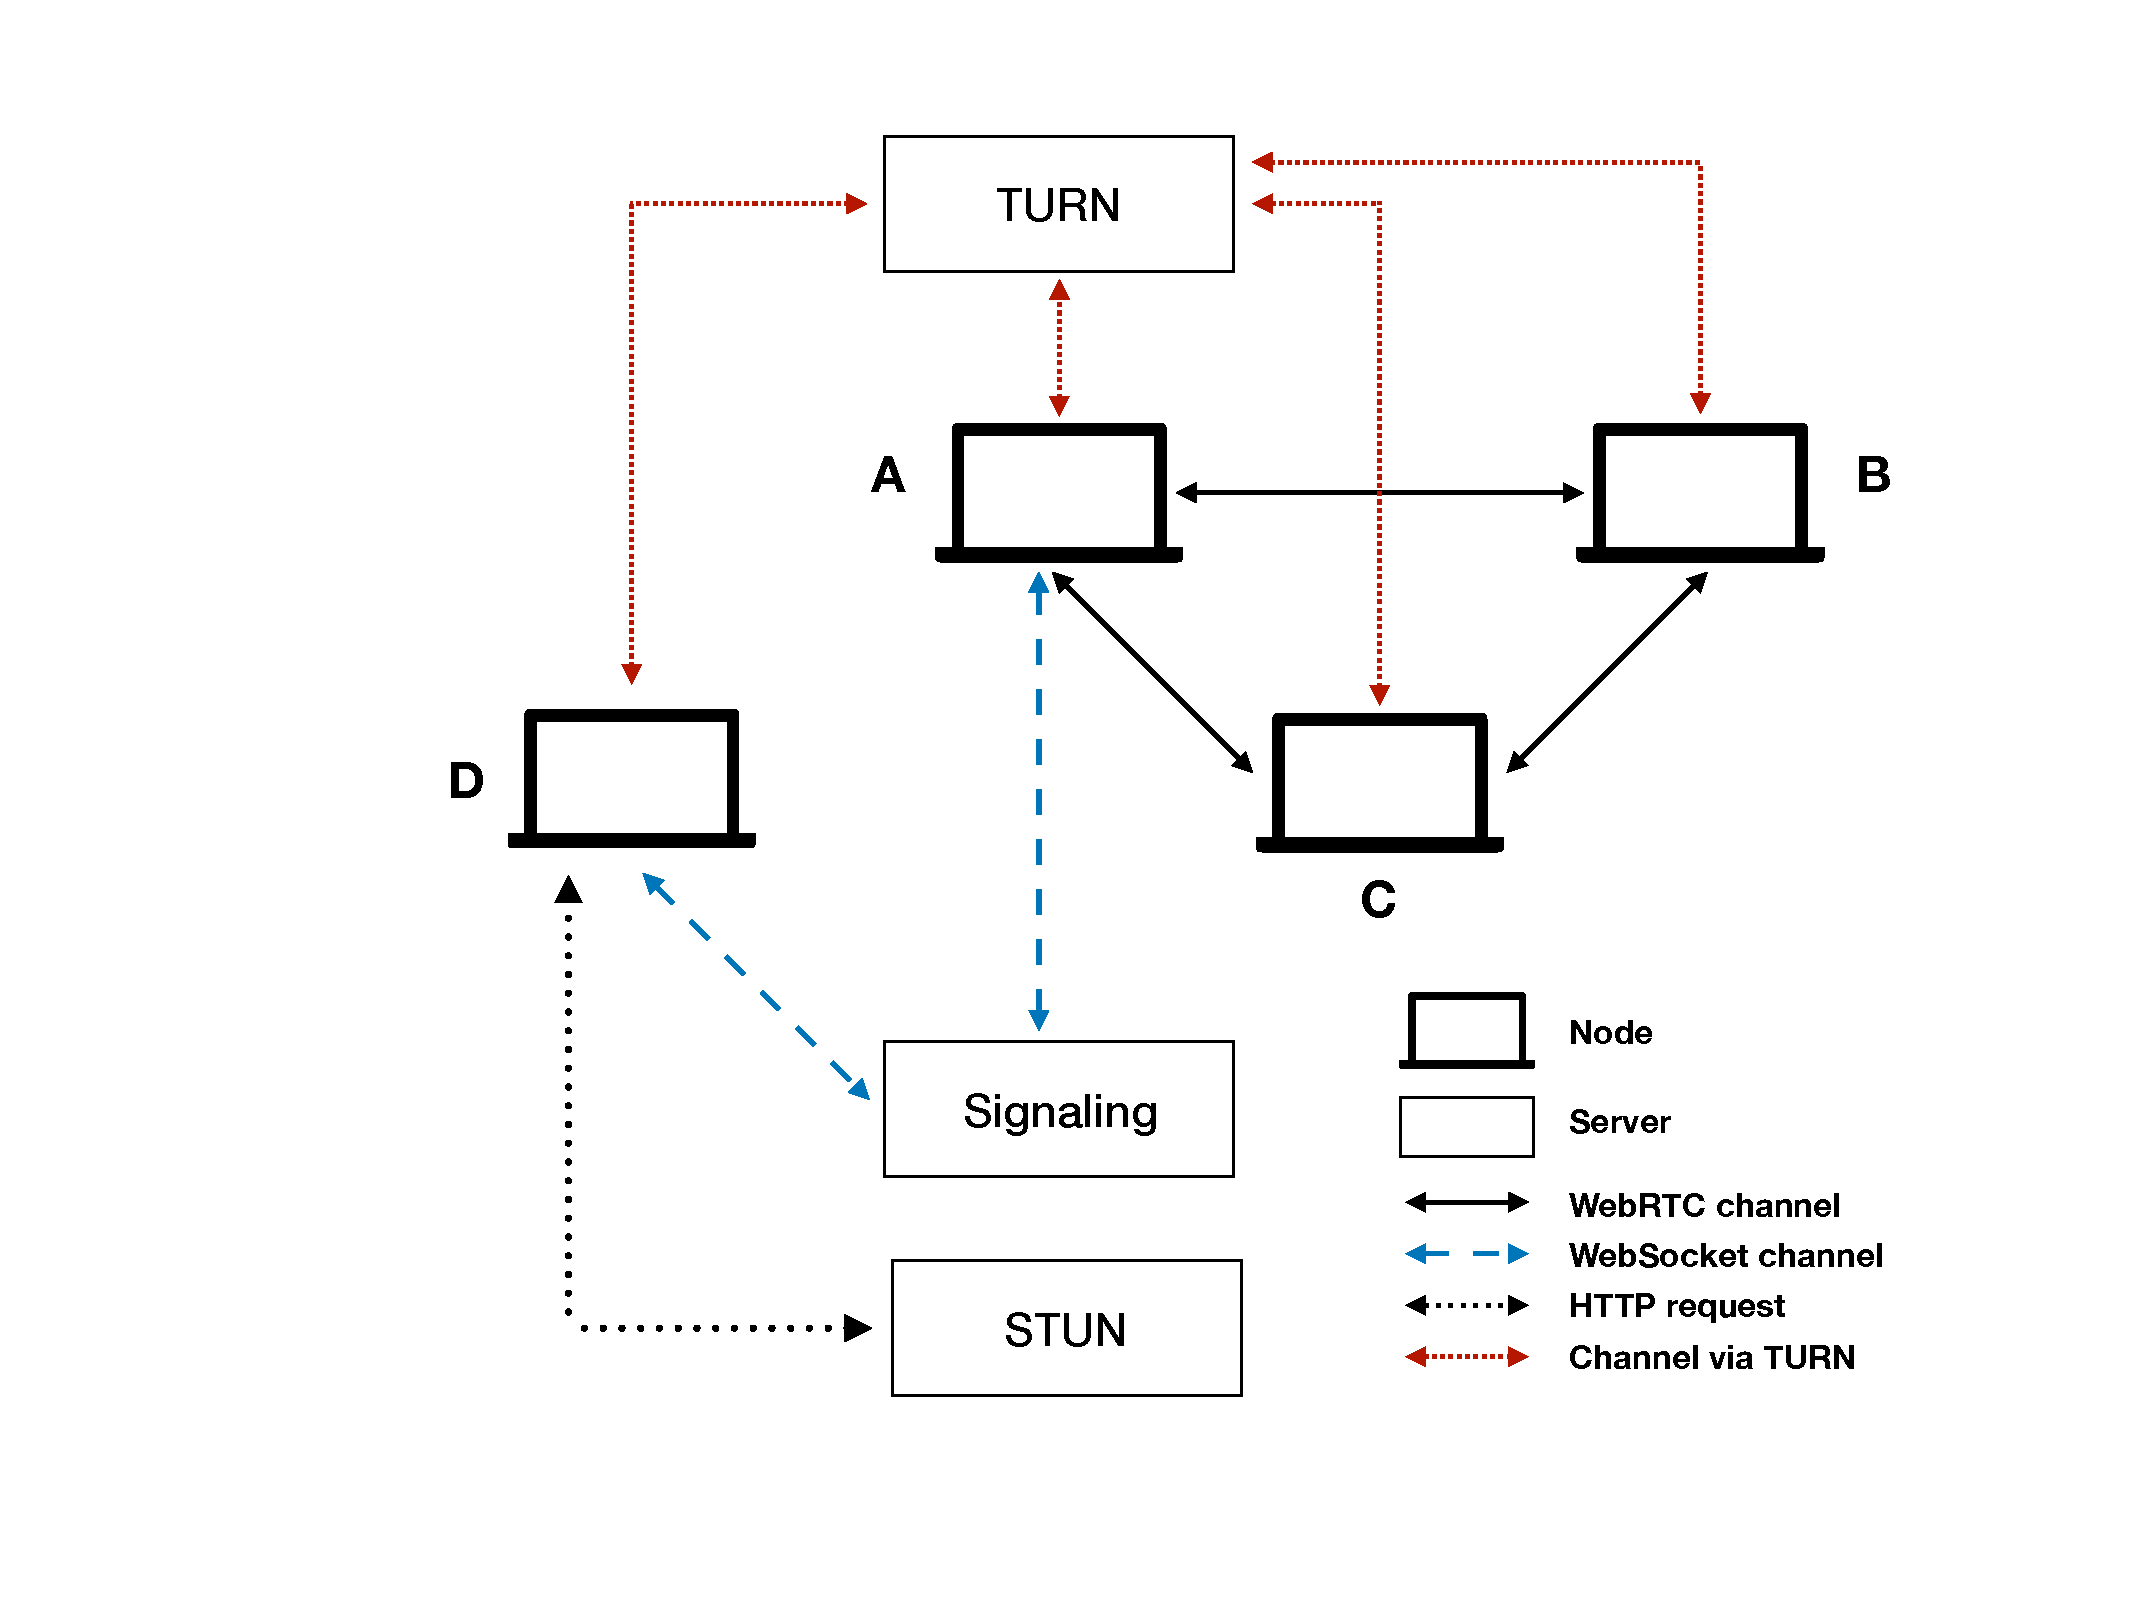
\includegraphics[page=1, trim=0cm 0cm 0cm 0cm, clip, width=.7\linewidth]{img/mute-figures.pdf}
  \caption{Architecture système de l'application MUTE}
  \label{fig:architecture-sys-mute}
\end{figure}

Plusieurs types de noeuds composent cette architecture.
Nous décrivons ci-dessous le type de chacun de ces noeuds ainsi que leurs rôles.

\subsubsection{Pairs}

Au centre de la collaboration se trouvent les noeuds qui correspondent aux utilisateur-rices de l'application et à leurs appareils.
Chaque noeud correspond à une instance de l'application \ac{MUTE}, \ie l'éditeur collaboratif de texte.
Chacun de ces noeuds peut donc consulter des documents et les modifier.

Ces noeuds forment un réseau \ac{P2P}, qui leur permet d'échanger directement notamment pour diffuser les modifications effectuées sur le document.
Les pairs interagissent aussi avec les autres types de noeuds, que nous décrivons dans les parties suivantes.

Notons qu'un noeud peut toutefois être déconnecté du système, \ie dans l'incapacité de se connecter aux autres pairs et d'interagir avec les autres types de noeuds.
Cela ne l'empêche toutefois pas l'utilisateur-rice d'utiliser \ac{MUTE}.

\subsubsection{Services réseaux}

Nous décrivons par cette appelation l'ensemble des composants nécessaires à l'établissement et le bon fonctionnement du réseau \ac{P2P} entre les appareils des utilisateur-rices.

Il s'agit de serveurs ayant pour buts de :
\begin{enumerate}
    \item Permettre à un pair d'obtenir les informations sur son propre état nécessaires pour l'établissement de connexions \ac{P2P}.
    \item Permettre à un pair de découvrir les autres pairs travaillant sur le même document et d'établir une connexion avec eux.
    \item Permettre à des pairs de communiquer même si leur configurations réseaux respectives empêchent l'établissement d'une connection \ac{P2P} directe.
\end{enumerate}

Nous détaillons plus précisément chacun de ces services et les interactions entre les pairs et ces derniers dans la \autoref{sec:mute-couche-reseau}.

\subsubsection{Services sécurité}

Nous décrivons par cette appelation l'ensemble des composants nécessaires à l'authentification des utilisateur-rices et à l'établissement de clés de groupe de chiffrement.

Il s'agit de serveurs ayant pour buts de :
\begin{enumerate}
    \item Permettre à un pair de s'authentifier.
    \item Permettre à un pair de faire connaître sa clé publique de chiffrement.
    \item Vérifier l'identité d'un pair.
    \item Permetttre à un pair de vérifier le comportement honnête du ou des serveurs servant les clés publiques de chiffrement.
\end{enumerate}

Nous dédions la \autoref{sec:mute-couche-securite} à la description de ces différents services et les interactions des pairs avec ces derniers.
